\chapter{Pricacy Pass}

\section{Introduction}
\subsection{Outline}

\begin{itemize}
    \item Introduction : Why do we need Privacy Pass?
    \begin{itemize}
        \item Websites need to tell humans and bots apart
        \item Goal and problems of human and servers.
        \item Existing solutions for the privacy
    \end{itemize}
    \item  Privacy Pass Architecture
    \begin{itemize}
        \item protocols
        \item Threat Model
    \end{itemize}
    \item  Privacy Pass Deployment models.
    \item Deploy
\end{itemize}


\subsection{Why do we need Privacy Pass?}
\begin{multicols}{2}
\subsubsection{Human Perspective}
\textbf{Goal:} Gain access to a service securely.

\textbf{Challenges:}
\begin{itemize}[topsep=0pt]
    \item Must prove they are real humans to the server.
    \item Do not want to compromise their privacy in the process.
\end{itemize}

\textbf{Proposed Solutions:}
\begin{itemize}[topsep=0pt]
    \item \textbf{MASQUE:} A protocol to provide privacy-preserving client identity for sensitive requests.
    \item \textbf{Privacy Pass:} Enables verification of legitimacy in a privacy-preserving manner.
\end{itemize}

\columnbreak

\subsubsection{Server Perspective}
\textbf{Goal:} Provide services only to legitimate users.

\textbf{Challenges:}
\begin{itemize}[topsep=0pt]
    \item Some bots are sophisticated enough to mimic real users.
    \item Ensuring smooth user experience without unnecessary hurdles.
\end{itemize}

\textbf{Existing Solutions and Their Limitations:}
\begin{itemize}[topsep=0pt]
    \item \textbf{CAPTCHA:} Difficult for bots but can be inconvenient for legitimate users, potentially affecting performance.
    \item \textbf{IP Filtering:} Effective at blocking malicious traffic but not privacy-friendly, as it often relies on tracking users.
\end{itemize}
\end{multicols}

\subsubsection{Conclusion}
Privacy Pass offers a middle ground by allowing servers to verify user legitimacy while maintaining user privacy, addressing the core needs of both humans and servers effectively.

\section{Privacy Pass Entities}
\begin{itemize}
    \item Token \textbf{Issuer} : Generates the tokens.
    \item \textbf{Origin} : The website/service.
    \begin{itemize}
        \item Needs to choose trusted Issuer. Send tokens challenges to Client.
        \item Verifies tokens received from Clients.
    \end{itemize}
    \item \textbf{Client} : Wants to authenticate to an Origin.
    \begin{itemize}
        \item Proves they have passed the challenge previously.
        \item Without needing to solve another challenge.
    \end{itemize}
    \item \textbf{Attester(s)} :
    \begin{itemize}
        \item Performs client property verification that is necessary for the issuance.
        \item Confirms, identifies or authenticates the Client.
    \end{itemize}
    \item \textbf{Token} : Unlinkable authenticators generated on the bases of authentication, attestation, or previous action.
\end{itemize}

\subsection{Interactions \& Privacy Requirements}
Context : Interactions and set of provided or available information between entities. 

\begin{itemize}
    \item \textbf{Redemption} context : (Client, Origin) $\rightarrow$ TokenChallenge , Origin name, Event timestamps, Client visible info
    \item \textbf{Issuance} context : (Client, Issuer, Attester) $\rightarrow$ Client identifiers. [Origin name]
    \item \textbf{Attestation} context : (Client, Attester) $\rightarrow$ Event timestamps
    \item\textbf{ Unlinkability} of a token : Cryptographic proofs allowing clients to authenticate to a server without;
    \begin{itemize}
        \item revealing identity or tracing the token back to the Issuer.
    \end{itemize}
\end{itemize}

\subsection{Trust Assumptions \& Threat Model}
\begin{figure}[H]
    \centering
    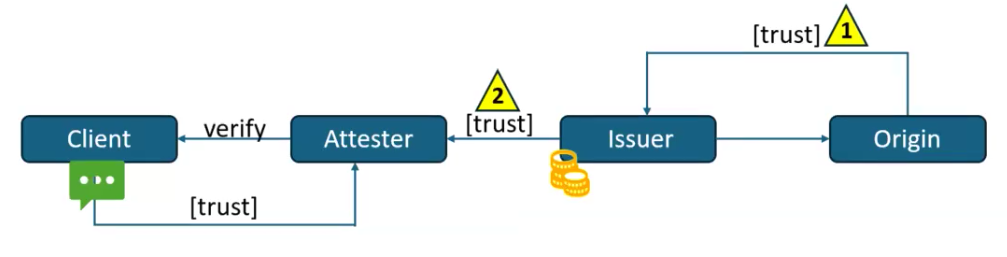
\includegraphics[width=0.8\textwidth]{img/trust assumptions.png}
    \caption{The 3 trust assumptions and 2 possible threats}
    \label{fig:trust assumptions}
\end{figure}

In figure \ref{fig:trust assumptions}, when the Client respond and the message pass between the Attester and the Issure we want to inforce the relation between the two with TLS or a digital signature. 


\section{Redemption Protocol}

The redemption protocol is an authorization mechanism that enables clients to present tokens to origins in order to gain access to services. The main aspects of the protocol are as follows:

\begin{itemize}
    \item Upon successful authorization, the requested service is granted to the client.
    \item Tokens may or may not correspond to the \texttt{TokenChallenge} (the challenge is sent by the origin to the client), depending on the specific issuance protocol and its configuration.
    \item The challenge provides the client with the necessary information required for successful use in the redemption context.
\end{itemize}


\subsection{Origin's Message: \texttt{TokenChallenge}}

The \texttt{TokenChallenge} serves as the mechanism for establishing the redemption context. The behavior varies based on the interaction type and the origin's configuration:

\begin{itemize}
    \item \textbf{Interactive:}
    \begin{itemize}
        \item A fresh and random redemption context is generated every time.
    \end{itemize}
    
    \item \textbf{Non-Interactive:}
    \begin{itemize}
        \item The redemption context is empty.
        \item Enables possible pre-fetching and caching of responses.
    \end{itemize}
    
    \item \textbf{Per-Origin Constraints:}
    \begin{itemize}
        \item Tokens are constrained to the origin that generated the challenge.
    \end{itemize}
    
    \item \textbf{Cross-Origin Constraints:}
    \begin{itemize}
        \item Requires explicit agreements to admit tokens issued by other origins in the set.
        \item Introduces challenges for managing token consumption across origins.
        \item Reusing the same token across origins risks breaking unlinkability.
    \end{itemize}
\end{itemize}

\section{Issuance Protocol}

The issuance protocol is responsible for producing token values that correspond to the \texttt{TokenChallenge}. It is described in RFC 9578, which outlines two variants of the protocol, both designed to operate over HTTP:

\begin{itemize}
    \item \textbf{Privately Verifiable:} Uses the issuer's secret key (\texttt{sk\_I}) and is based on an Oblivious Pseudorandom Function (OPRF).
    \item \textbf{Publicly Verifiable:} Uses the issuer's public key (\texttt{pk\_I}) and relies on a blind RSA signature scheme.
\end{itemize}

The protocol involves interactions between the client and the issuer through two main components:
\begin{itemize}
    \item \textbf{\texttt{TokenRequest}:} The client initiates the issuance by sending a request to the issuer.
    \item \textbf{\texttt{TokenResponse}:} The issuer processes the request and responds with the necessary data to complete the issuance.
\end{itemize}

The client computes the token using a one-round protocol. This process involves:
\begin{itemize}
    \item \textbf{Attestation:} The client interacts with the attester to gather the required information.
    \item Using the \texttt{TokenRequest} and \texttt{TokenResponse} messages to finalize the computation.
\end{itemize}

\begin{boxH}
    This kind of authentication can be used at different leves, like user level, machine level, process level
\end{boxH}

\section{Possible Attesting Procedures}

To ensure the legitimacy of clients and eliminate automated or fraudulent entities, several attesting procedures can be employed:

\subsection{Bot or Automated Client Elimination}
\begin{itemize}
    \item \textbf{CAPTCHA:}, Stands for \textbf{Completely Automated Public Turing test to tell Computers and Humans Apart}.
    \item Challenges clients with tasks that are simple for humans but difficult for bots to solve.
\end{itemize}

\subsection{Device-Level Attestation}
\begin{itemize}
    \item Relies on trusted hardware to authenticate client devices.
    \item For example, \textbf{Apple Private Access Tokens} use secure device-level attestations to confirm authenticity.
\end{itemize}

\subsection{Client State Verification}
Client state can be verified by checking specific attributes, such as:
\begin{itemize}
    \item \textbf{Geographical Information:} Validating the client's location.
    \item \textbf{Application Layer Account:} Ensuring the client has a valid account uniquely identifiable at the application layer.
\end{itemize}

These procedures collectively enhance security by verifying client authenticity while maintaining usability for legitimate users.

\section{Deployment Models: Terms and Requirements}

Deployment models define the context and constraints under which systems operate, with a focus on protecting unlinkability. Key terms and requirements include:

\subsection{Collusion}
The sharing of context information between entities, which affects unlinkability:
\begin{itemize}
    \item \textbf{Split Architecture:} Assumes no collusion between entities, ensuring the preservation of unlinkability.
    \item \textbf{Joint and Shared Architectures:} Entities are able to collude, which may compromise unlinkability.
\end{itemize}

\subsection{Unlinkability}
Unlinkability is critical to maintaining privacy across interactions and must be preserved between the following entities:
\begin{itemize}
    \item \textbf{Origin and Client:} Preventing the origin from linking client activities.
    \item \textbf{Issuer and Client:} Ensuring the issuer cannot trace tokens back to specific clients.
    \item \textbf{Attester and Origin:} Protecting the origin from correlating information provided by the attester.
\end{itemize}

These requirements highlight the importance of deployment models in safeguarding privacy and minimizing information sharing between entities.


\subsubsection{Split Attester, Issuer, and Origin}
\begin{itemize}[topsep=0pt]
    \item The most general deployment model
    \item Attester, Issuer, Origin has separate views about the Client.
    \item Attester, potentially sees sensitive client information.
    \item Issuer receive the tokenRequest from the trusted Attester.
    \item Trust relationship between the Issuer and Attester
    \begin{itemize}
        \item Dependents on the issuance protocol.
     \end{itemize}
    \item Any type of token challenge is possible since
    \begin{itemize}
        \item the attestation, issuance, and redemption contexts are separate.
    \end{itemize}
\end{itemize}